\chapter{Two dimensional reconstruction}
\label{APP::ELLIPT}

As shown in section~\ref{SEC::ANALYSIS::2D}, the expression for
\textit{disp(size,length,width)} can be expanded in terms of the
ellipticity parameter $\epsilon=1-width/length$, 
\[disp = a_1(size,length)\times \epsilon + a_2(size,length)\times
\epsilon^2 + \cdots.\]
We further assume that the dependence on $length$ is of secondary
importance with respect to $size$,
\[disp = \sum_1^\infty a_i(size)\times\epsilon^i\]

Optimization of $a_i(size)$ is done with simulated \Gray events,
selected with energy in proportion to the Crab Nebula spectrum. The
images have artificial night-sky noise added and are analyzed in the
same manner as real events as described in
sections~\ref{SEC::ANALYSIS::CONDITIONING},
\ref{SEC::ANALYSIS::PARAMETERIZATION} and
\ref{SEC::ANALYSIS::DATASELECTION}. Events are binned in terms of 
$\log(size/U)$, where $U=1622\,DC/deg$ describes the characteristic
light density per unit arc length in a muon image
\citep{REF::HORAN::2001THESIS}. For each bin, the best fit for the
following two functions are found,
\begin{eqnarray}
disp^{(1)} & = & a_1\,\times\,\epsilon \label{EQN::APPELLIPT::LINEAR}\\
disp^{(2)} & = & a_1\,\times\,\epsilon\,+\,a_2\,\times\,\epsilon^2 \label{EQN::APPELLIPT::QUADRATIC}
\end{eqnarray}
Figure~\ref{FIG::APPELLIPT::FITS} shows the distribution of $distance$
vs.  $\epsilon$ for simulated events in two $size$ bins. It can be
seen from the diagrams that the quadratic fit,
eqn.~\ref{EQN::APPELLIPT::QUADRATIC}, is not reasonable as $\epsilon$
increases, as it turns over and begins to decrease. The fitted
function $a_1(size)$ and the quality of the fits are shown in
figure~\ref{FIG::APPELLIPT::ELLIPTANDCHISQ}. It can be seen that,
$a_1(size)$ can be approximated by
\begin{equation}
a_1(size)=1.36^\circ\,+\,0.14^\circ\times\log(size/U) \label{EQN::APPELLIPT::A1}
\end{equation}

\begin{figure}[p]
\begin{minipage}{0.5\textwidth}\centerline{$Size/U=0.55$}\end{minipage}%
\begin{minipage}{0.5\textwidth}\centerline{$Size/U=5.5$}\end{minipage}\\[-1.5ex]
\resizebox*{0.5\textwidth}{!}{\rotatebox{270}{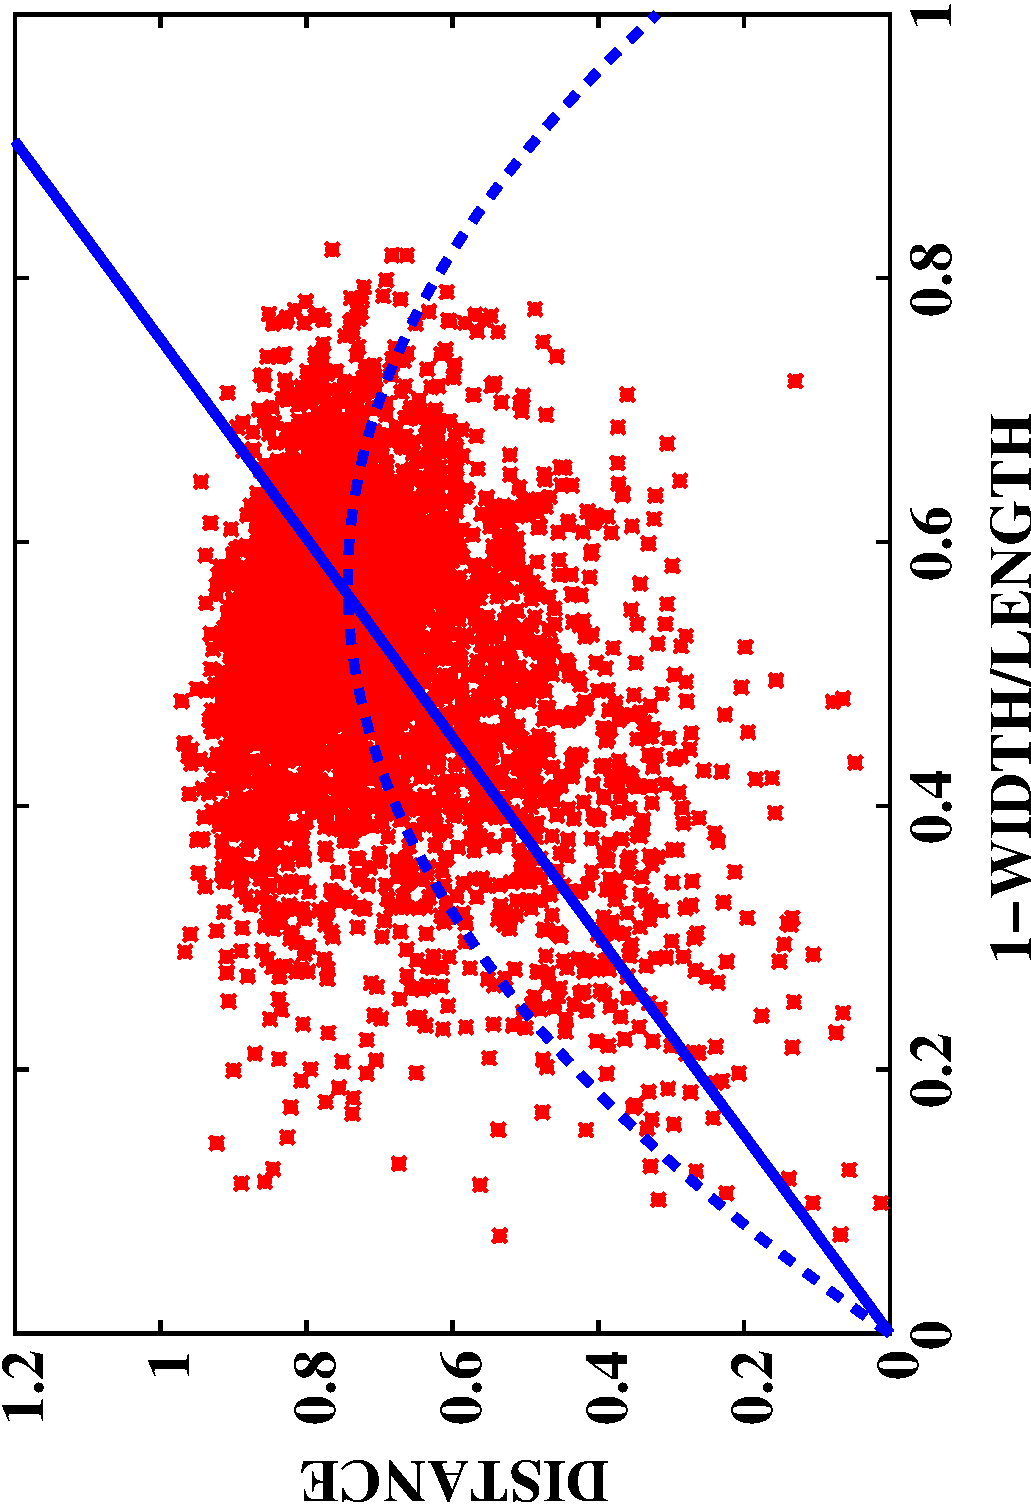
\includegraphics[draft=false]{plots/app-ellipt/fits2.pdf}}}%
\resizebox*{0.5\textwidth}{!}{\rotatebox{270}{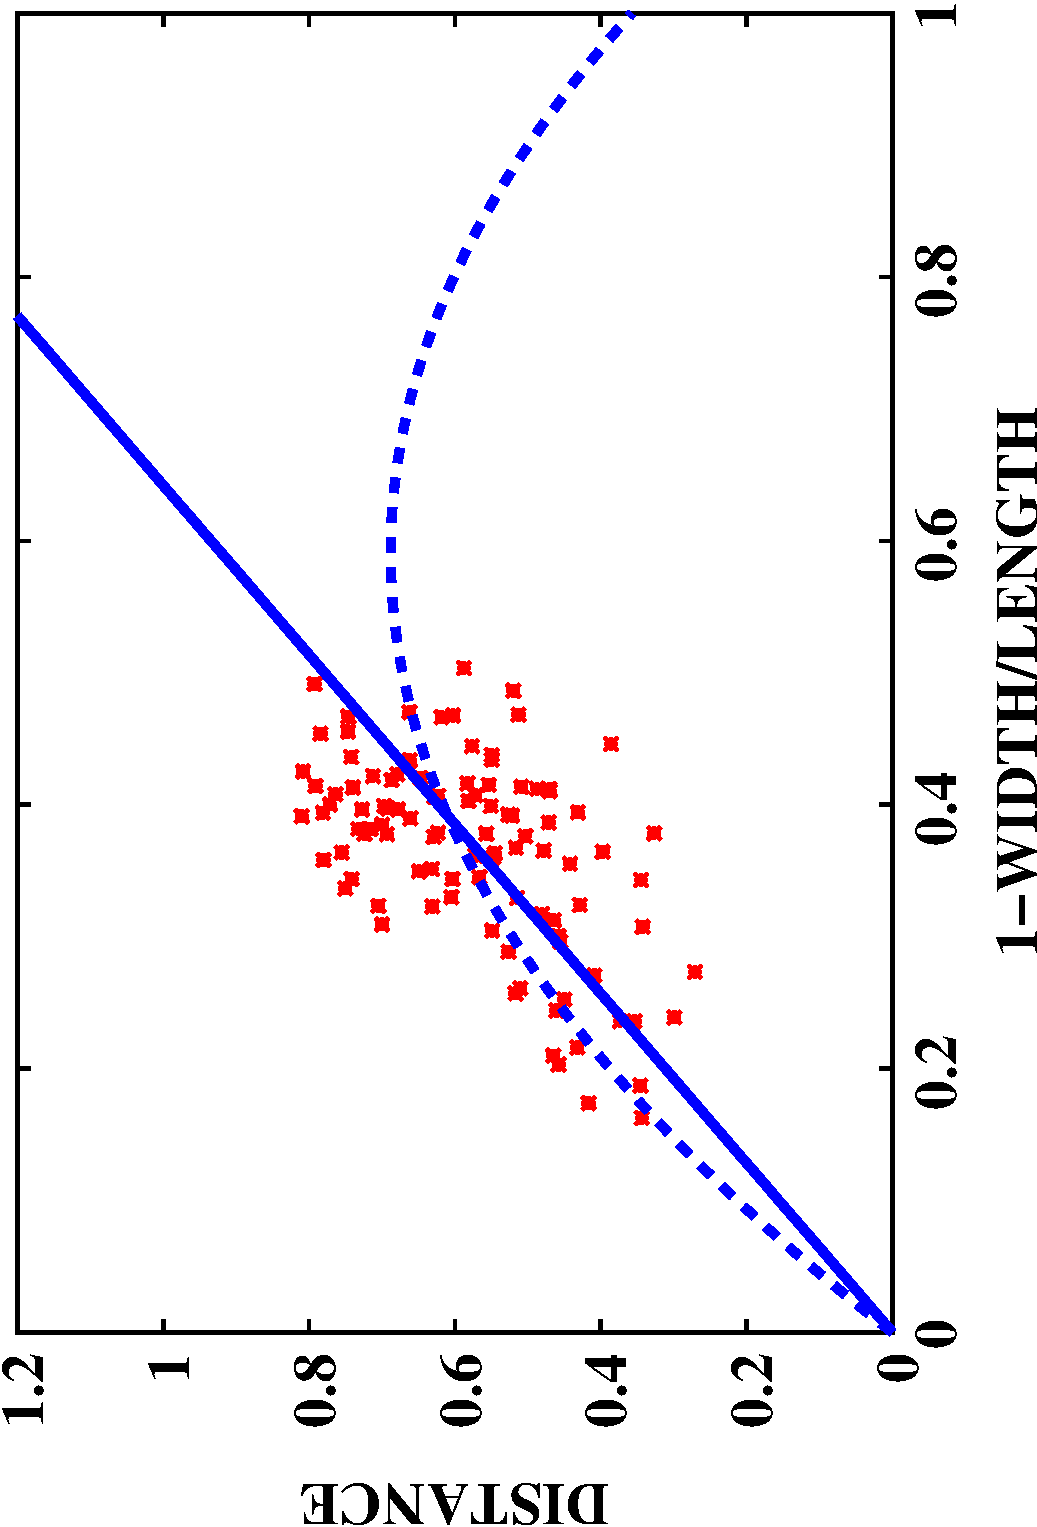
\includegraphics[draft=false]{plots/app-ellipt/fits4.pdf}}}
\caption{\label{FIG::APPELLIPT::FITS} Optimization of $disp$ with 
simulated \Gray events, in two energy bins. The $distance$ of centroid
from source is on the y-axis, the ellipticity, $\epsilon$, on the
x-axis. The best fit for eqn.~\ref{EQN::APPELLIPT::LINEAR} and
\ref{EQN::APPELLIPT::QUADRATIC} are shown.}
\end{figure}

\begin{figure}[p]
\resizebox*{0.5\textwidth}{!}{\rotatebox{0}{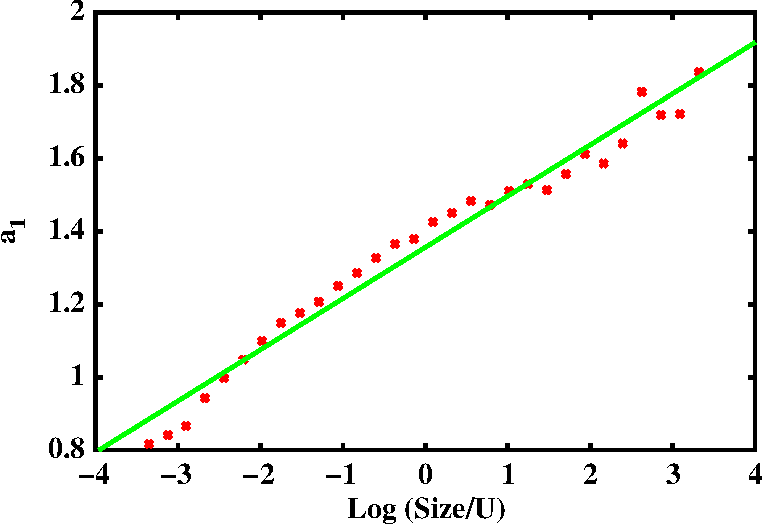
\includegraphics[draft=false]{plots/app-ellipt/ellipt.pdf}}}%
\resizebox*{0.5\textwidth}{!}{\rotatebox{0}{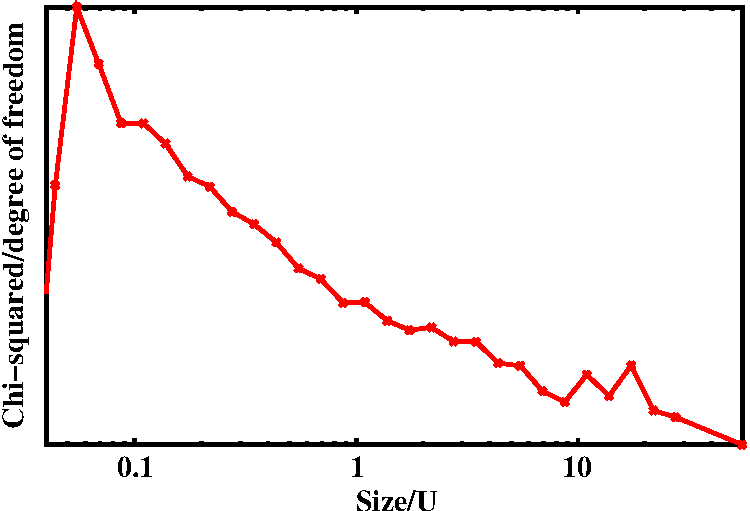
\includegraphics[draft=false]{plots/app-ellipt/chisq.pdf}}}
\caption{\label{FIG::APPELLIPT::ELLIPTANDCHISQ} (Left) Best fit of 
parameter $a_1$ from eqn.~\ref{EQN::APPELLIPT::LINEAR} to simulated data.
The function $a_1(size)$ can itself be fit by a linear relationship of
$a_1(size)=1.36^\circ\,+\,0.14^\circ\times\log(size/U)$. (Right) $\chi^2$
per degree of freedom for fit of $a_1$ to simulated events.}
\end{figure}
\clearpage

Using the relationship given in eqn.~\ref{EQN::APPELLIPT::A1}, the
arrival direction of the simulated events can reconstructed using the
two dimensional technique. Since the origin of the simulated \Grays is
known, the performance of the reconstruction can be
evaluated. Distributions of the longitudinal and transverse error in
the reconstructed arrival direction (as illustrated in
figure~\ref{FIG::APPELLIPT::RECONSTRUCTIONERRORS}) are shown in
figure~\ref{FIG::APPELLIPT::ERRORDISTRIBUTIONS}. The distribution of
longitudinal error has an r.m.s. width of
$\sigma_\parallel\approx0.23^\circ$ and can be fit by a Gaussian with
$\sigma_{G}\approx0.19^\circ$. The distribution of transverse error
has width of $\sigma_\perp\approx0.22^\circ$. 

High energy events have considerably better reconstruction
characteristics, a cut of $\log(size/U)>1.0$, which keeps only 1\% of
the events, gives $\sigma_\parallel\approx0.15^\circ$ and
$\sigma_\perp\approx0.05^\circ$, as shown in
figure~\ref{FIG::APPELLIPT::ERRORVSSIZE}. This suggests that a high
energy cut will will result in a sky-map with better angular
resolution.

\begin{figure}[t]
\centerline{\resizebox*{\textwidth}{!}{\rotatebox{0}{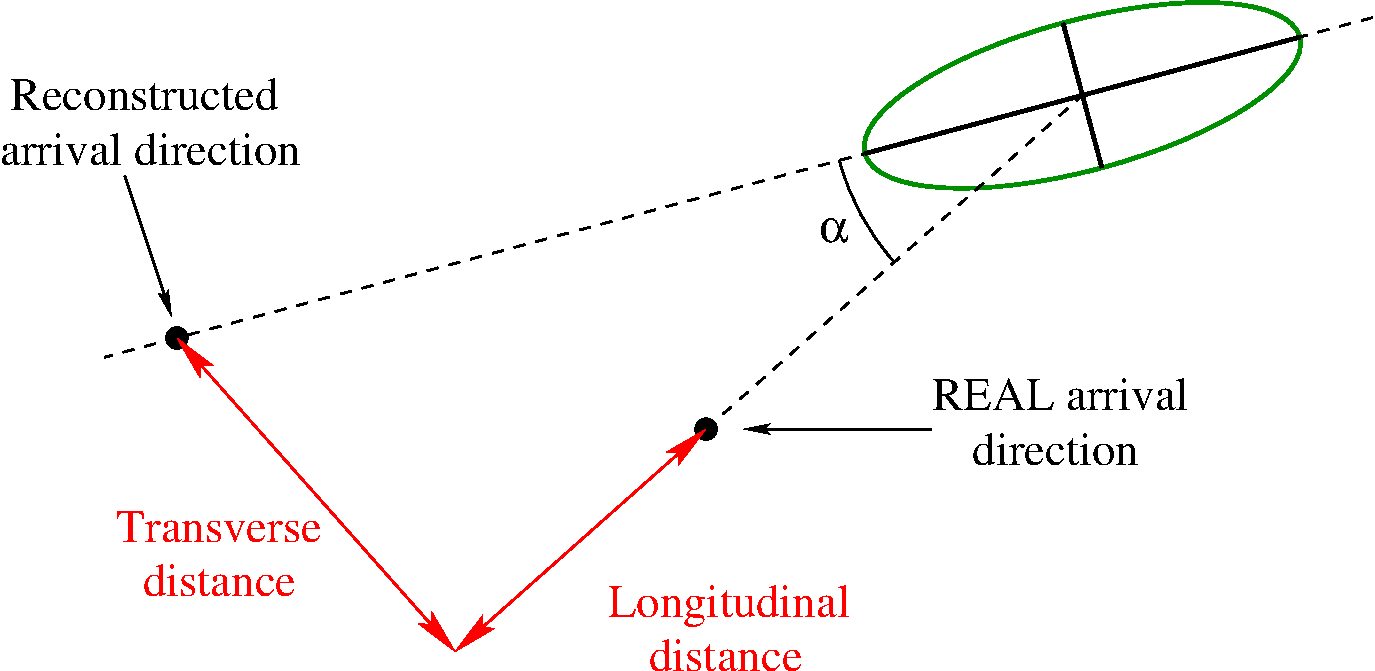
\includegraphics[draft=false]{plots/app-ellipt/arrival_direction.pdf}}}}
\caption{\label{FIG::APPELLIPT::RECONSTRUCTIONERRORS} Illustration of the
longitudinal and transverse errors in reconstructing the arrival direction
of \Gray events.}
\end{figure}

\begin{figure}[p]
\resizebox*{0.5\textwidth}{!}{\rotatebox{0}{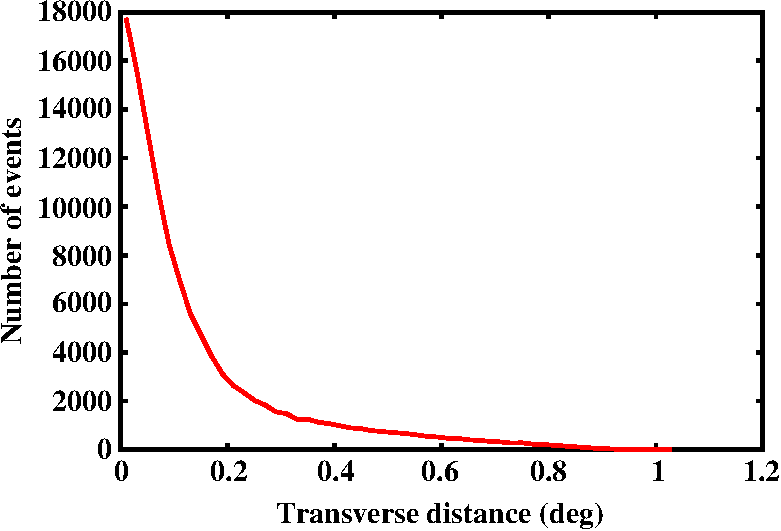
\includegraphics[draft=false]{plots/app-ellipt/trans.pdf}}}%
\resizebox*{0.5\textwidth}{!}{\rotatebox{0}{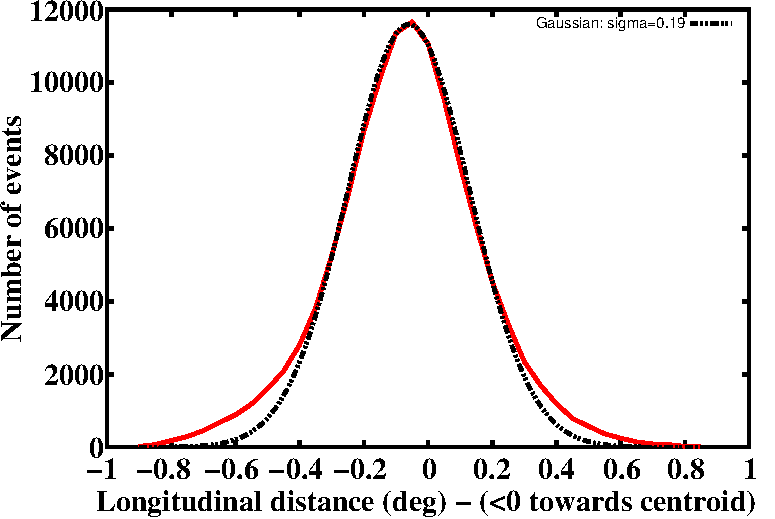
\includegraphics[draft=false]{plots/app-ellipt/long+gauss.pdf}}}
\caption{\label{FIG::APPELLIPT::ERRORDISTRIBUTIONS} Distribution of 
transverse (left) and longitudinal (right) error in reconstructing
the arrival direction of simulated events.}
\end{figure}

\begin{figure}[p]
\centerline{\resizebox*{\textwidth}{!}{\rotatebox{0}{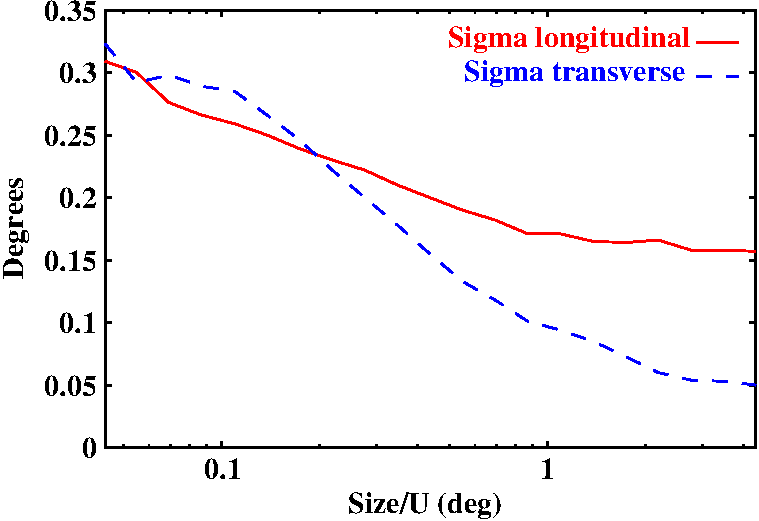
\includegraphics[draft=false]{plots/app-ellipt/estimateBySize+dist09.pdf}}}}
\caption{\label{FIG::APPELLIPT::ERRORVSSIZE} Dependence of longitudinal
($\sigma_\parallel$) and transverse ($\sigma_\perp$) error on $size$
cut imposed. }
\end{figure}
